\chapter{Feature representation}
\label{chap-features}

Linear regression and classification are powerful tools, but in the real world, data often
exhibit {\em non-linear} behavior that cannot immediately be
captured by the linear models which we have built so far.  For example,
suppose the true behavior of a system (with $d=2$) looks like this
wavelet:\note{This plot is of the so-called {\em jinc}
function $J_1(\rho)/\rho$ for $\rho^2=x_1^2 + x_2^2$}
%
% Note rho is radial distance squared, because we don't want to have to use
% a sqrt in the polynomial basis

\centerline{\includegraphics[width=0.5\textwidth]{figures/regression_features1_sombrero_comp1.pdf}}

\noindent
Such behavior is actually ubiquitous in physical systems, e.g., in the
vibrations of the surface of a drum, or scattering of light through an
aperture.  However, no single hyperplane would be a very good fit to
such peaked responses!

A richer class of hypotheses can be obtained by performing a
non-linear feature transformation $\phi(x)$ before doing the
regression. That is, $\theta^Tx + \theta_0$ is a linear function of
$x$, but $\theta^T\phi(x) + \theta_0$ is a non-linear function of $x,$
if $\phi$ is a non-linear function of $x$.

There are many different ways to construct $\phi$.  Some are
relatively systematic and domain independent.
Others are directly related to the semantics (meaning) of the original
features, and we construct them deliberately with our application (goal) in mind.

%%%%%%%%%%%%%%%%%%%%%%%%%%%%%%%%%%%%%%%%%%%%%%%%%%%%%%%%%%%%%%%%%%%%%%%%%%%%%
\section{Gaining intuition about feature transformations}

\label{sec-features_classifiers}

In this section, we explore the effects of non-linear feature
transformations on simple classification problems, to gain intuition.



% There is no linear separator for this two-dimensional dataset!  But, we have a trick
% available:  take a low-dimensional data set and move it, using a
% non-linear transformation into a higher-dimensional space, and look
% for a linear separator there.

Let's look at an example data set that starts in 1-D:

\begin{examplebox}
  \begin{center}
    \begin{tikzpicture}
      \draw [<->, gray] (-3,0) -- (3,0)
      node [black, right] {$x$};
      \draw [gray] (0,.6) -- (0,-.6)
      node [black, below] {0};

      \pic at (-1.5, 0) {plusblk};
      \pic at (-.5, 0) {minusblk};
      \pic at (.5, 0) {minusblk};
      \pic at (1.5, 0) {plusblk};

    \end{tikzpicture}
  \end{center}
\end{examplebox}

These points are not linearly separable,\note{What's a linear
  separator for data in 1D?  A point!}  but consider the
transformation $\phi(x) = [x,x^2]^T$. Putting the data in $\phi$ space,
we see that it is now separable.  There are lots of possible
separators;  we have just shown one of them here.

\begin{examplebox}
  \begin{center}
    \begin{tikzpicture}
      \draw [<->, gray] (-3,0) -- (3,0)
      node [black, right] {$x$};
      \draw [<->, gray] (0,-.6) -- (0,4)
      node [black, above] {$x^2$};

      \draw [dashed] (-3, 1.25) -- (3, 1.25)
      node [below, xshift=-1cm] {separator};

      \pic at (-1.5, 2.25) {plusblk};
      \pic at (-.5, .25) {minusblk};
      \pic at (.5, .25) {minusblk};
      \pic at (1.5, 2.25) {plusblk};

    \end{tikzpicture}
  \end{center}
\end{examplebox}

A linear separator in $\phi$ space is a nonlinear separator in the
original space!  Let's see how this plays out in our simple example.
Consider the separator $x^2  - 1 = 0$, which labels the half-plane
$x^2 -1 > 0$ as positive.  What separator does it correspond to in the
original 1-D space?
We have to ask the question:  which $x$ values have the property that
$x^2 - 1 = 0$.  The answer is $+1$ and $-1$, so those two points
constitute our separator, back in the original space.  And we can use
the same reasoning to find the region of 1D space that is labeled
positive by this separator.

\begin{examplebox}
  \begin{center}
    \begin{tikzpicture}
      \draw [<->, gray] (-3,0) -- (3,0)
      node [black, right] {$x$};
      \draw [gray] (0,.6) -- (0,-.6)
      node [black, below] {0};
      \draw [gray] (1,.2) -- (1,-.2)
      node [black, below] {1};
      \draw [gray] (-1,.2) -- (-1,-.2)
      node [black, below] {-1};

      \fill (1,0) circle (2.5pt);
      \fill (-1,0) circle (2.5pt);

      \draw[decoration={calligraphic brace,amplitude=5pt}, decorate, line width=1.25pt]
      (-2.95,0.2) node {} -- (-1.05,0.2);
      \draw[decoration={calligraphic brace,amplitude=5pt}, decorate, line width=1.25pt]
      (-.95,0.2) node {} -- (.95,0.2);
      \draw[decoration={calligraphic brace,amplitude=5pt}, decorate, line width=1.25pt]
      (1.05,0.2) node {} -- (2.95,0.2);

      \pic at (-2, 0.7) {plus};
      \pic at (0, 0.7) {minus};
      \pic at (2, 0.7) {plus};

    \end{tikzpicture}
  \end{center}
\end{examplebox}




%%%%%%%%%%%%%%%%%%%%%%%%%%%%%%%%%%%%%%%%%%%%%%%%%%%%%%%%%%%%%%%%%%%%%%%%%%%%%
\section{Systematic feature construction}
Here are two different ways to systematically construct features in a
  {\em problem independent} way.

\subsection{Polynomial basis}

\label{polyBasis}

If the features in your problem are already naturally numerical, one
systematic strategy for constructing a new feature space is to use a
  {\em polynomial basis}\index{basis functions!polynomial basis}.  The idea is that, if you are using the
$k$th-order basis (where $k$ is a positive integer), you include a
feature for every possible product of $k$ different dimensions in your
original input.

Here is a table illustrating the $k$th order polynomial basis for
different values of $k$, calling out the cases when $d=1$ and $d>1$:

\begin{center}
  \begin{tabular}{c c c}
    Order  & $d=1$             & in general ($d>1$)       \\
    \hline
    0      & $[1]$             & $[1]$                    \\
    1      & $[1,x]^T$         & $[1,x_1, \ldots, x_d]^T$ \\
    2      & $[1,x,x^2]^T$     & $[1,x_1, \ldots, x_d,
    x_1^2, x_1x_2, \ldots]^T$                             \\
    3      & $[1,x,x^2,x^3]^T$ & $[1,x_1, \ldots,
          x_1^2, x_1x_2, \ldots,
    x_1x_2x_3, \ldots]^T$                                 \\
    \vdots & \vdots            & \vdots
  \end{tabular}
\end{center}

This transformation can be used in combination with linear regression
or logistic regression (or any other regression or classification
model).  When we're using a linear regression or classification model,
the key insight is that a linear regressor or separator in the {\em
    transformed space} is a non-linear regressor or separator in the
original space.


% (* capture jinc function with features *)
% 
% npts = 1000;
% SeedRandom[1];
% x1 = RandomReal[{-rm, rm}, {npts}]; 
% x2 = RandomReal[{-rm, rm}, {npts}]; 
% r = (x1)^2 + (x2)^2;
% yv = BesselJ[1, r]/r;
% pts = Transpose@{x1, x2, yv};
% model = LinearModelFit[
%    pts, {  1, 
%     Subscript[x, 1]^2 + 
%      Subscript[x, 2]^2, (Subscript[x, 1]^2 + Subscript[x, 2]^2)^2,
%     (Subscript[x, 1]^2 + Subscript[x, 2]^2)^4}, { Subscript[x, 1], 
%     Subscript[x, 2]}];
% 
% vp = {1.207331108916506`, -3.0537082213398925`, 0.8168339441793491`};
% 
% p1 = ListPointPlot3D[ pts, 
%    AxesLabel -> {Subscript[x, 1], Subscript[x, 2], y}, 
%    PlotRange -> {0, 0.6}, ViewPoint -> vp ];
% p3 = Plot3D[
%    model[Subscript[x, 1], Subscript[x, 2]], {Subscript[x, 1], -rm, 
%     rm}, {Subscript[x, 2], -rm, rm}, PlotStyle -> Opacity[0.2], 
%    PlotRange -> {0, 0.6}, PlotPoints -> 100];
% p4 = Show[{p1, p3}];
% gr1 = GraphicsRow[{p1, p4}, ImageSize -> Large]
% Export["regression_features2_fitsombrero.png", gr1, 
%   ImageResolution -> 1200]; 

For example, the wavelet pictured at the start of this chapter can be
fit much better than with just a hyperplane, using linear regression
with polynomials up to order $k=8$:\note{Specifically, this
  example uses $[1, x_1, x_2, x_1^2 + x_2^2, (x_1^2 + x_2^2)^2, (x_1^2 + x_2^2)^4]^T$ }

\centerline{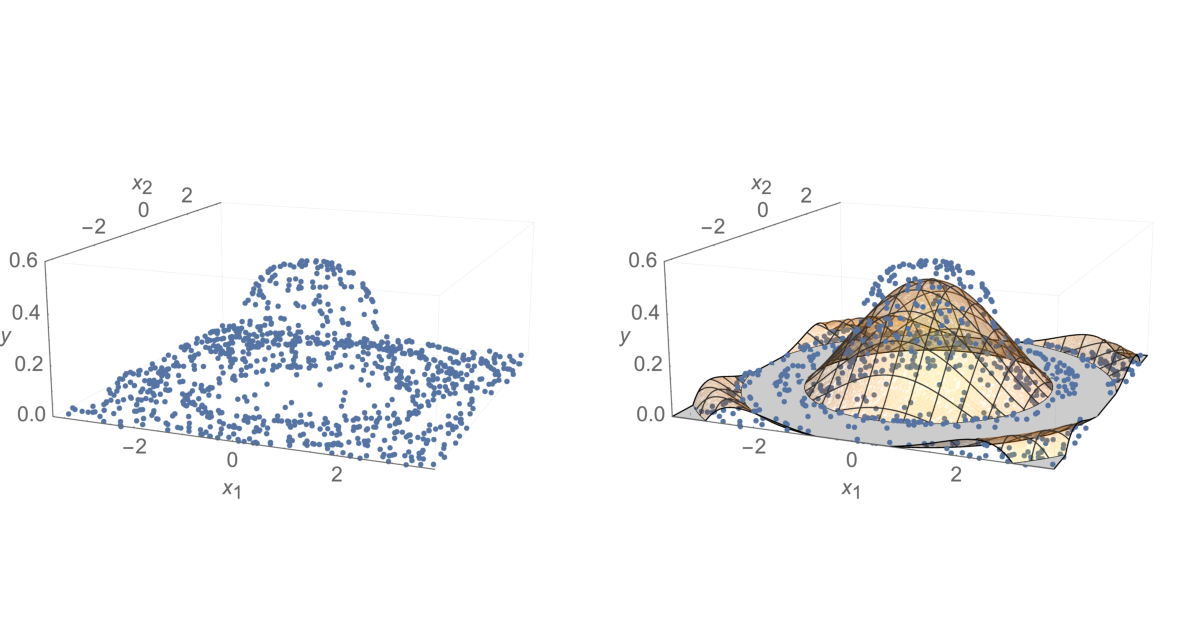
\includegraphics[width=0.9\textwidth]{figures/regression_features2_fitsombrero.pdf}}

\noindent
The raw data (with $n=1000$ random samples) is plotted on the left, and the regression result (curved surface) is on the right.

% \question{
% What polynomial terms would be needed for a good basis of features, if the wavelet were centered somewhere other than at the origin?
% }

Now let's look at a classification example and see how polynomial feature transformation may help us.

One well-known example is the ``exclusive or'' ({\sc xor}) data set, the drosophila\note{D. Melanogaster is a species of fruit fly, used as a simple system in which to study genetics, since 1910.} of machine-learning data sets:

\begin{examplebox}
  \begin{center}
    \begin{tikzpicture}
      \pic at (-1, -1) {plusblk};
      \pic at (-1, +1) {minusblk};
      \pic at (+1, -1) {minusblk};
      \pic at (+1, +1) {plusblk};
    \end{tikzpicture}
  \end{center}
\end{examplebox}

Clearly, this data set is not linearly separable. So, what if we try to solve the {\sc xor} classification problem using a polynomial
basis as the feature transformation?  We can just take our
two-dimensional data and transform it into a higher-dimensional data
set, by applying $\phi$.  Now, we have a classification problem as
usual.

Let's try it for $k = 2$ on our {\sc xor} problem.  The feature
transformation is
\[\phi([x_1, x_2]^T) = [1, x_1, x_2, x_1^2, x_1 x_2, x_2^2]^T\;\;.\]
\question{
  If we train a classifier after performing this feature
  transformation, would we lose any expressive
  power if we let $\theta_0 = 0$ (i.e., trained without offset instead of
  with offset)?}
We might run a classification learning algorithm and find a separator
with coefficients $\theta = [0, 0, 0, 0, 4, 0]^T$ and $\theta_0 = 0$.
This corresponds to
\[0 + 0 x_1 + 0 x_2 + 0 x_1^2 + 4 x_1 x_2 + 0x_2^2 + 0 = 0\]
and is plotted below, with the gray shaded region classified as
negative and the white region classified as positive:
\begin{examplebox}
  \begin{center}
    % 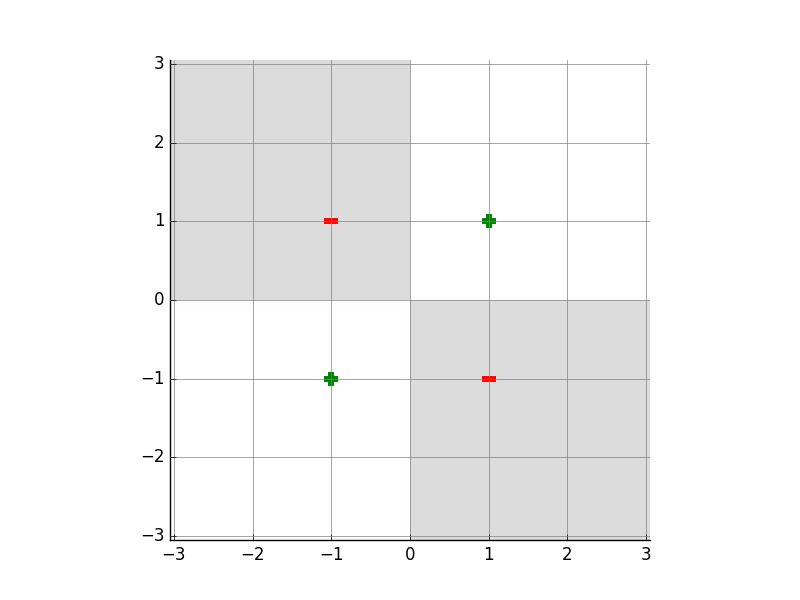
\includegraphics[scale=0.3]{figures/feature_representation_1.png}
    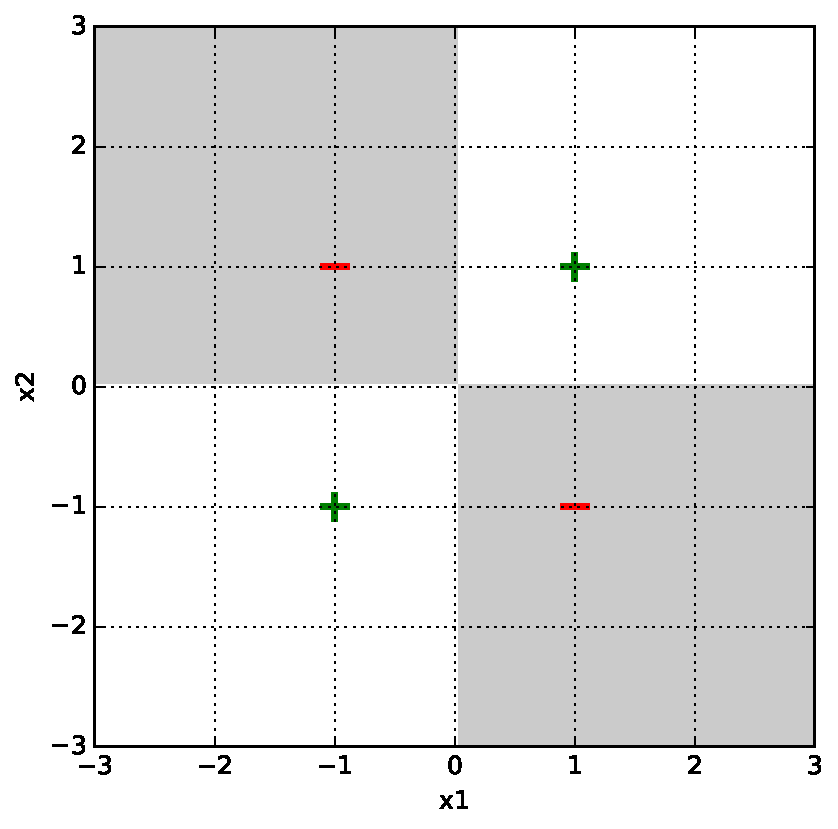
\includegraphics[scale=0.48]{figures/feature_representation_xor_sign.pdf}
  \end{center}
\end{examplebox}
\question{
  Be sure you understand why this high-dimensional hyperplane is a
  separator, and how it corresponds to the figure.}

For fun, we show some more plots below.  Here is another result for a
linear classifier on {\sc xor} generated with logistic regression and
gradient descent, using a random initial starting point and second-order
polynomial basis:

\begin{examplebox}
  \begin{center}
    % 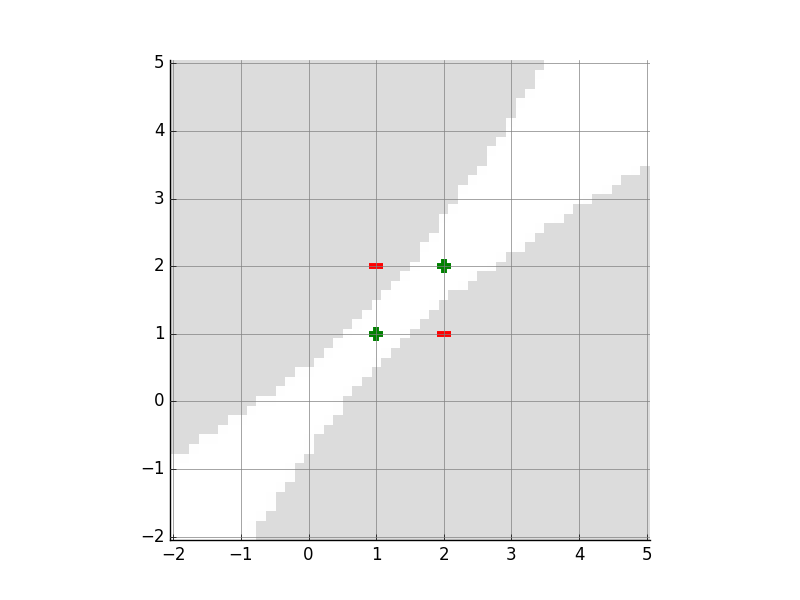
\includegraphics[scale=0.3]{figures/feature_representation_2.png}
    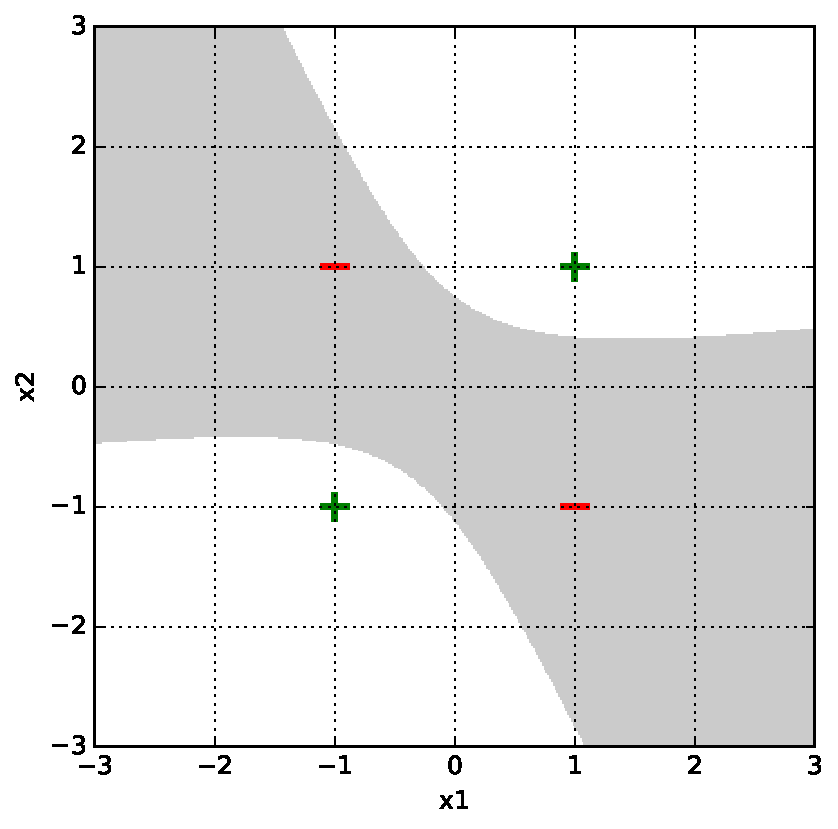
\includegraphics[scale=0.48]{figures/feature_representation_xor_order2.pdf}
  \end{center}
\end{examplebox}

Here is a harder data set.  Logistic regression with gradient descent
failed to separate it with a second, third, or fourth-order basis feature
representation, but succeeded with a fifth-order basis.
Shown below are some results after $\sim1000$
gradient descent iterations (from random starting points) for bases of
order 2 (upper left), 3 (upper right), 4 (lower left), and 5 (lower right).
\begin{examplebox}
  \begin{center}
    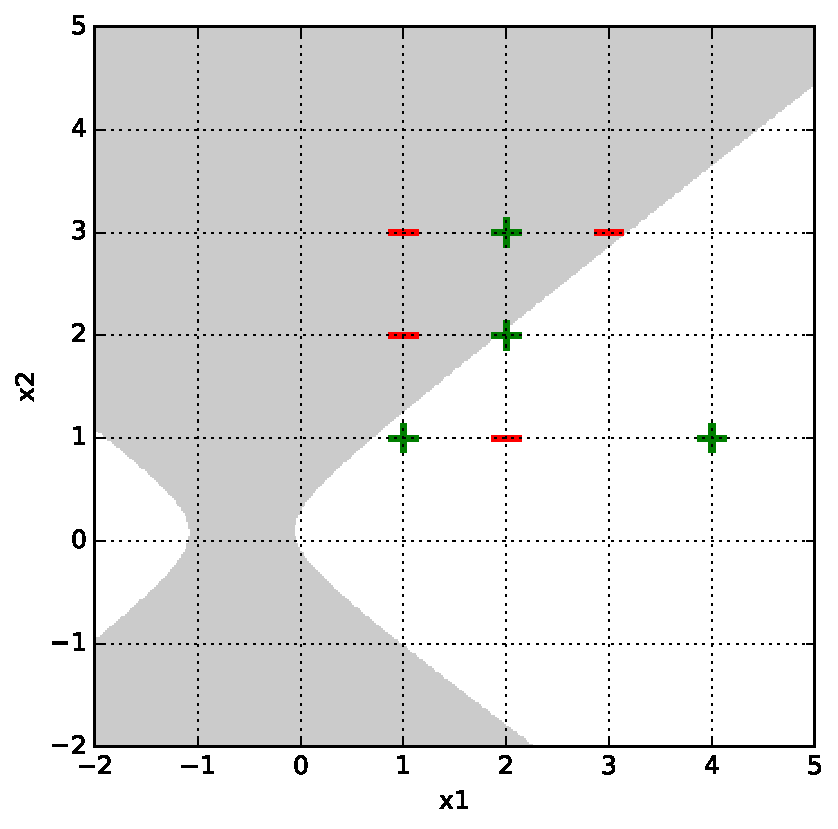
\includegraphics[width=0.48\linewidth]{figures/feature_representation_hard_order2.pdf}
    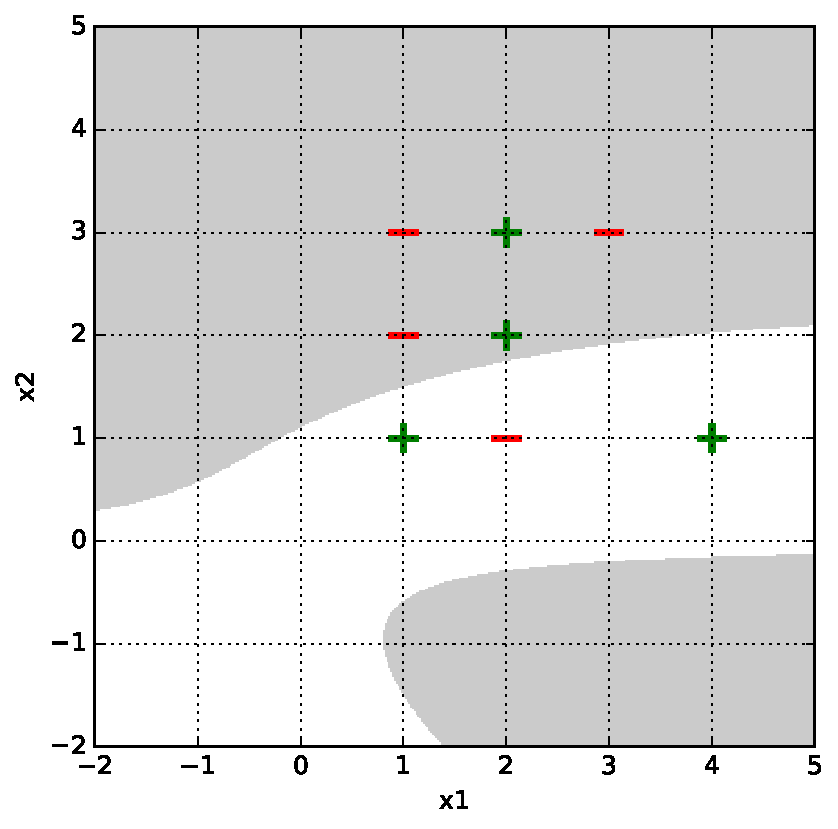
\includegraphics[width=0.48\linewidth]{figures/feature_representation_hard_order3.pdf} \\
    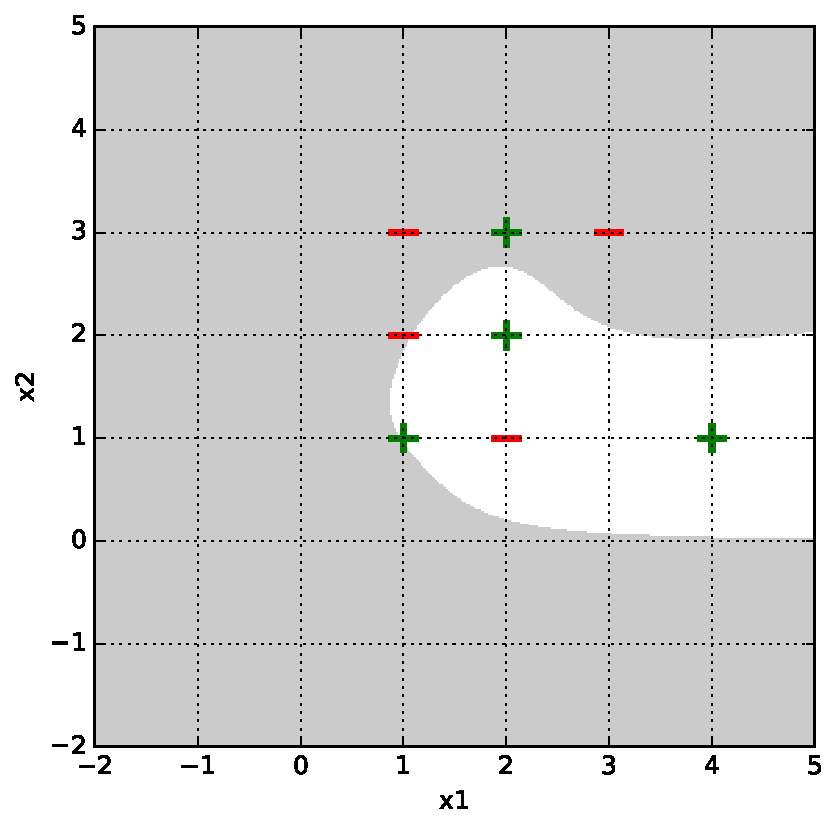
\includegraphics[width=0.48\linewidth]{figures/feature_representation_hard_order4.pdf}
    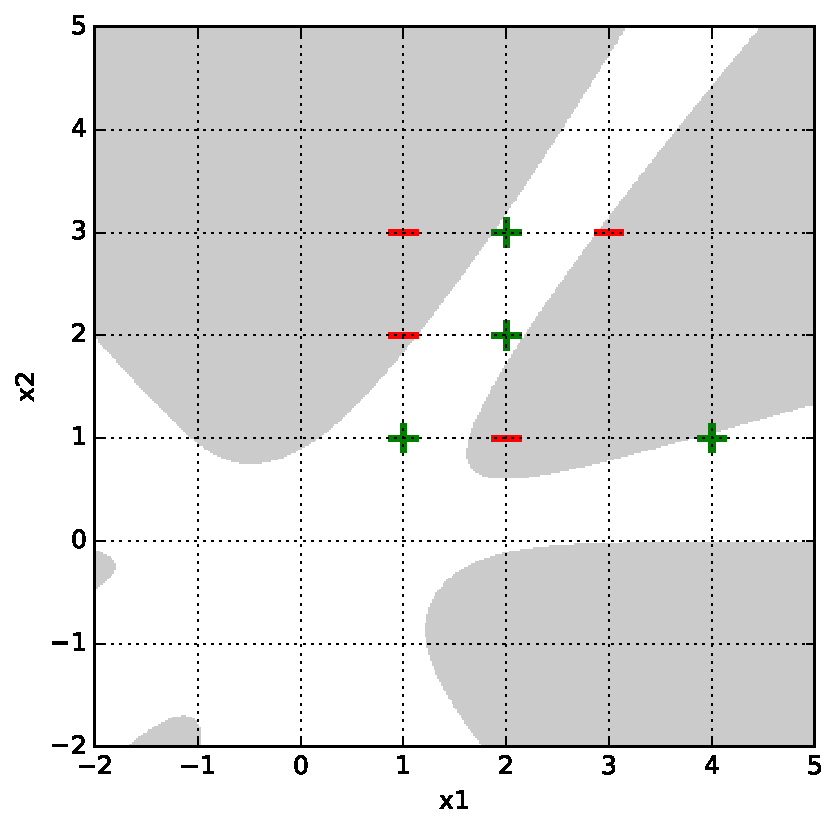
\includegraphics[width=0.48\linewidth]{figures/feature_representation_hard_order5.pdf}
  \end{center}
\end{examplebox}

\question{
Percy Eptron has a domain with four numeric input features, $(x_1,
  \ldots, x_4)$.  He decides to use a representation of the form
\[\phi(x) = {\rm PolyBasis}((x_1, x_2), 3) ^\frown
{\rm PolyBasis}((x_3, x_4), 3)\]
where $a^\frown b$ means the vector $a$ concatenated with the vector
$b$.   What is the dimension of Percy's representation?  Under what
assumptions about the original features is this a reasonable choice?
}


%%%%%%%%%%%%%%%%%%%%%%%%%%%%%%%%%%%%%%%%%%%%%%%%%%%%%%%%%%%%%%%%%%%%%%%%%%%%%

\subsection{Radial basis functions}
\index{basis functions!radial basis}
Another cool idea is to use {\em the training data itself} to
construct a feature space.  The idea works as follows.  For any
particular point $p$ in the input space $\mathcal{X}$, we can construct a feature
$f_p$ which takes any element $x \in \mathcal{X}$ and returns a
scalar value that is related to how far $x$ is from the $p$ we started
with.

Let's start with the basic case, in which $\mathcal{X} = \R^d$.  Then
we can define
\[f_p(x) = e^{-\beta\norm{p - x}^2}\;\;.\]
This function is maximized when $p = x$ and decreases exponentially as
$x$ becomes more distant from $p$.

The parameter $\beta$ governs how
quickly the feature value decays as we move away from the center point
$p$.  For large values of $\beta$, the $f_p$ values are nearly 0
almost everywhere except right near $p$;  for small values of $\beta$,
the features have a high value over a larger part of the space.

\question{What is $f_p(p)$?}

Now, given a dataset $\data$ containing $n$ points, we can make a
feature transformation $\phi$ that maps points in our original
space, $\R^d$, into points in a new space, $\R^n$.  It is defined as
follows:
\[\phi(x) = [f_{\ex{x}{1}}(x), f_{\ex{x}{2}}(x), \ldots,
  f_{\ex{x}{n}}(x)]^T\;\;.\]
So, we represent a new datapoint $x$ in terms of how far it is from
each of the datapoints in our training set.

This idea can be generalized in several ways and is the fundamental
concept underlying {\em kernel methods}\index{kernel methods}, that
you should read about some time. This idea of describing objects in
terms of their similarity to a set of reference objects is very
powerful and can be applied to cases where $\mathcal{X}$ is not a
simple vector space, but where the inputs are graphs or strings or
other types of objects, as long as there is a distance metric defined
on it.

%TODO:  Add rbf logistic regression plots

\section{Hand-constructing features for real domains}

\label{handBuiltFeatures}
In many machine-learning applications, we are given descriptions of
the inputs with many different types of attributes, including numbers,
words, and discrete features.  An important factor in the success of
an ML application is the way that the features are chosen to be encoded
by the human who is framing the learning problem.

\subsection{Discrete features}
Getting a good encoding of discrete features is particularly
important.  You want to create ``opportunities'' for the ML system to
find the underlying regularities.  Although there are machine-learning
methods that have special mechanisms for handling discrete inputs,
most of
the methods we consider in this class will assume the input vectors
$x$ are in $\R^d$.  So, we have to figure out some reasonable
strategies for turning discrete values into (vectors of) real numbers.

We'll start by listing some encoding strategies, and then work through
some examples. Let's assume we have some feature in our raw data that
can take on one of $k$ discrete values.
\begin{itemize}
  \item{\bf Numeric:}  Assign each of these values a number, say $1.0/k,
          2.0/k, \ldots, 1.0$.  We might want to then do some further processing, as
        described in Section~\ref{realFeatures}.  This is a sensible
        strategy {\em only} when the discrete values really do signify some
        sort of numeric quantity, so that these numerical values are meaningful.\index{hand-built features!numeric}

  \item{\bf Thermometer code:}  If your discrete values have a natural
        ordering, from $1, \ldots, k$, but not a natural mapping into real
        numbers, a good strategy is to use a vector of length $k$ binary
        variables, where we convert discrete input value $0 < j \leq k$ into
        a vector in which the first $j$ values are $1.0$ and the rest are
        $0.0$.  This does not necessarily imply anything about the spacing
        or numerical quantities of the inputs, but does convey something
        about ordering.\index{hand-built features!thermometer}

  \item{\bf Factored code:}  If your discrete values can sensibly be
        decomposed into two parts (say the ``maker'' and ``model'' of a car),
        then it's best to treat those as two separate features, and choose
        an appropriate encoding of each one from this list.\index{hand-built features!factored}

  \item{\bf One-hot code:}  If there is no obvious numeric, ordering, or
        factorial structure, then the best strategy is to use a vector of
        length $k$, where we convert discrete input value $0 < j \leq k$
        into a vector in which all values are $0.0$, except for the $j$th,
        which is $1.0$.\index{hand-built features!one-hot}

  \item{\bf Binary code:} It might be tempting for the computer
        scientists among us to use some binary code, which would let us
        represent $k$ values using a vector of length $\log k$.  {\em This
            is a bad idea!}  Decoding a binary code takes a lot of work, and
        by encoding your inputs this way, you'd be forcing your system to
          {\em learn} the decoding algorithm.\index{hand-built features!binary code}
\end{itemize}

As an example, imagine that we want to encode blood types, that are
drawn from the set $\{A+, A-, B+, B-, AB+, AB-, O+, O-\}$.  There is
no obvious linear numeric scaling or even ordering to this set.  But
there is a reasonable {\em factoring}, into two features: $\{A, B, AB,
  O\}$ and $\{+, -\}$.  And, in fact, we can further reasonably factor
the first group into $\{A, {\rm not}A\}$, $\{B, {\rm not}B\}$.\note{It
  is sensible (according to Wikipedia!) to treat $O$ as having neither
  feature $A$ nor feature $B$.}  So, here are two plausible encodings
of the whole set:
\begin{itemize}
  \item Use a 6-D vector, with two components of the vector each encoding the
        corresponding factor using a one-hot encoding.
  \item Use a 3-D vector, with one dimension for each factor, encoding
        its presence as $1.0$ and absence as $-1.0$ (this is sometimes
        better than $0.0$).  In this case, $AB+$ would be $[1.0, 1.0, 1.0]^T$
        and $O-$ would be $[-1.0, -1.0, -1.0]^T$.
\end{itemize}
\question{How would you encode $A+$ in both of these approaches?}

\subsection{Text}
The problem of taking a text (such as a tweet or a product review, or
even this document!) and encoding it as an input for a
machine-learning algorithm is interesting and complicated.  Much later
in the class, we'll study sequential input models, where, rather than
having to encode a text as a fixed-length feature vector, we feed it
into a hypothesis word by word (or even character by character!).

There are some simple encodings that work well for basic
applications.  One of them is the {\em bag of words} ({\sc bow})
model. \index{hand-built features!text encoding} The idea is to let $d$ be the number of words in our
vocabulary (either computed from the training set or some other body
of text or dictionary).  We will then make a binary vector (with
values $1.0$ and $0.0$) of length $d$, where element $j$ has value
$1.0$ if word $j$ occurs in the document, and $0.0$ otherwise.

\subsection{Numeric values}
\label{realFeatures}
If some feature is already encoded as a numeric value (heart rate,
stock price, distance, etc.) then we should generally keep it as a
numeric value.   An exception might be a situation in which we know
there are natural ``breakpoints'' in the semantics:  for example,
encoding someone's age in the US, we might make an explicit
distinction between under and over 18 (or 21), depending on what kind
of thing we are trying to predict.   It might make sense to divide
into discrete bins (possibly spacing them closer together for the very
young) and to use a one-hot encoding for some sorts of medical situations
in which we don't expect a linear (or even monotonic) relationship
between age and some physiological features.

If we choose to leave a feature as numeric, it is typically useful to
  {\em scale} it, so that it tends to be in the range $[-1, +1]$.
Without performing this transformation, if we have one feature with
much larger values than another, it will take the learning algorithm a
lot of work to find parameters that can put them on an equal basis.
We could also perform a more involved scaling/transformation
$\phi(x) = \dfrac{x - \overline{x}}{\sigma}$, where $\overline{x}$
is the average of the $\ex{x}{i}$, and $\sigma$ is the standard deviation of
the $\ex{x}{i}$.  The resulting feature values will have mean $0$ and
standard deviation $1$.   This transformation is sometimes called {\em
    standardizing} a variable.\note{Such standard variables are often known as
  ``z-scores,'' for example, in the social sciences.}

Then, of course, we might apply a higher-order polynomial-basis
transformation to one or more groups of numeric features.

\question{
  Consider using a polynomial basis of order $k$ as a feature
  transformation $\phi$ on our data.  Would increasing $k$ tend to
  increase or decrease structural error?  What about estimation error?
}



%%% Local Variables:
%%% mode: latex
%%% TeX-master: "top"
%%% End:
